\subsection{DSM Prototype: Local-edge Domain}

\begin{figure}[tbp]
	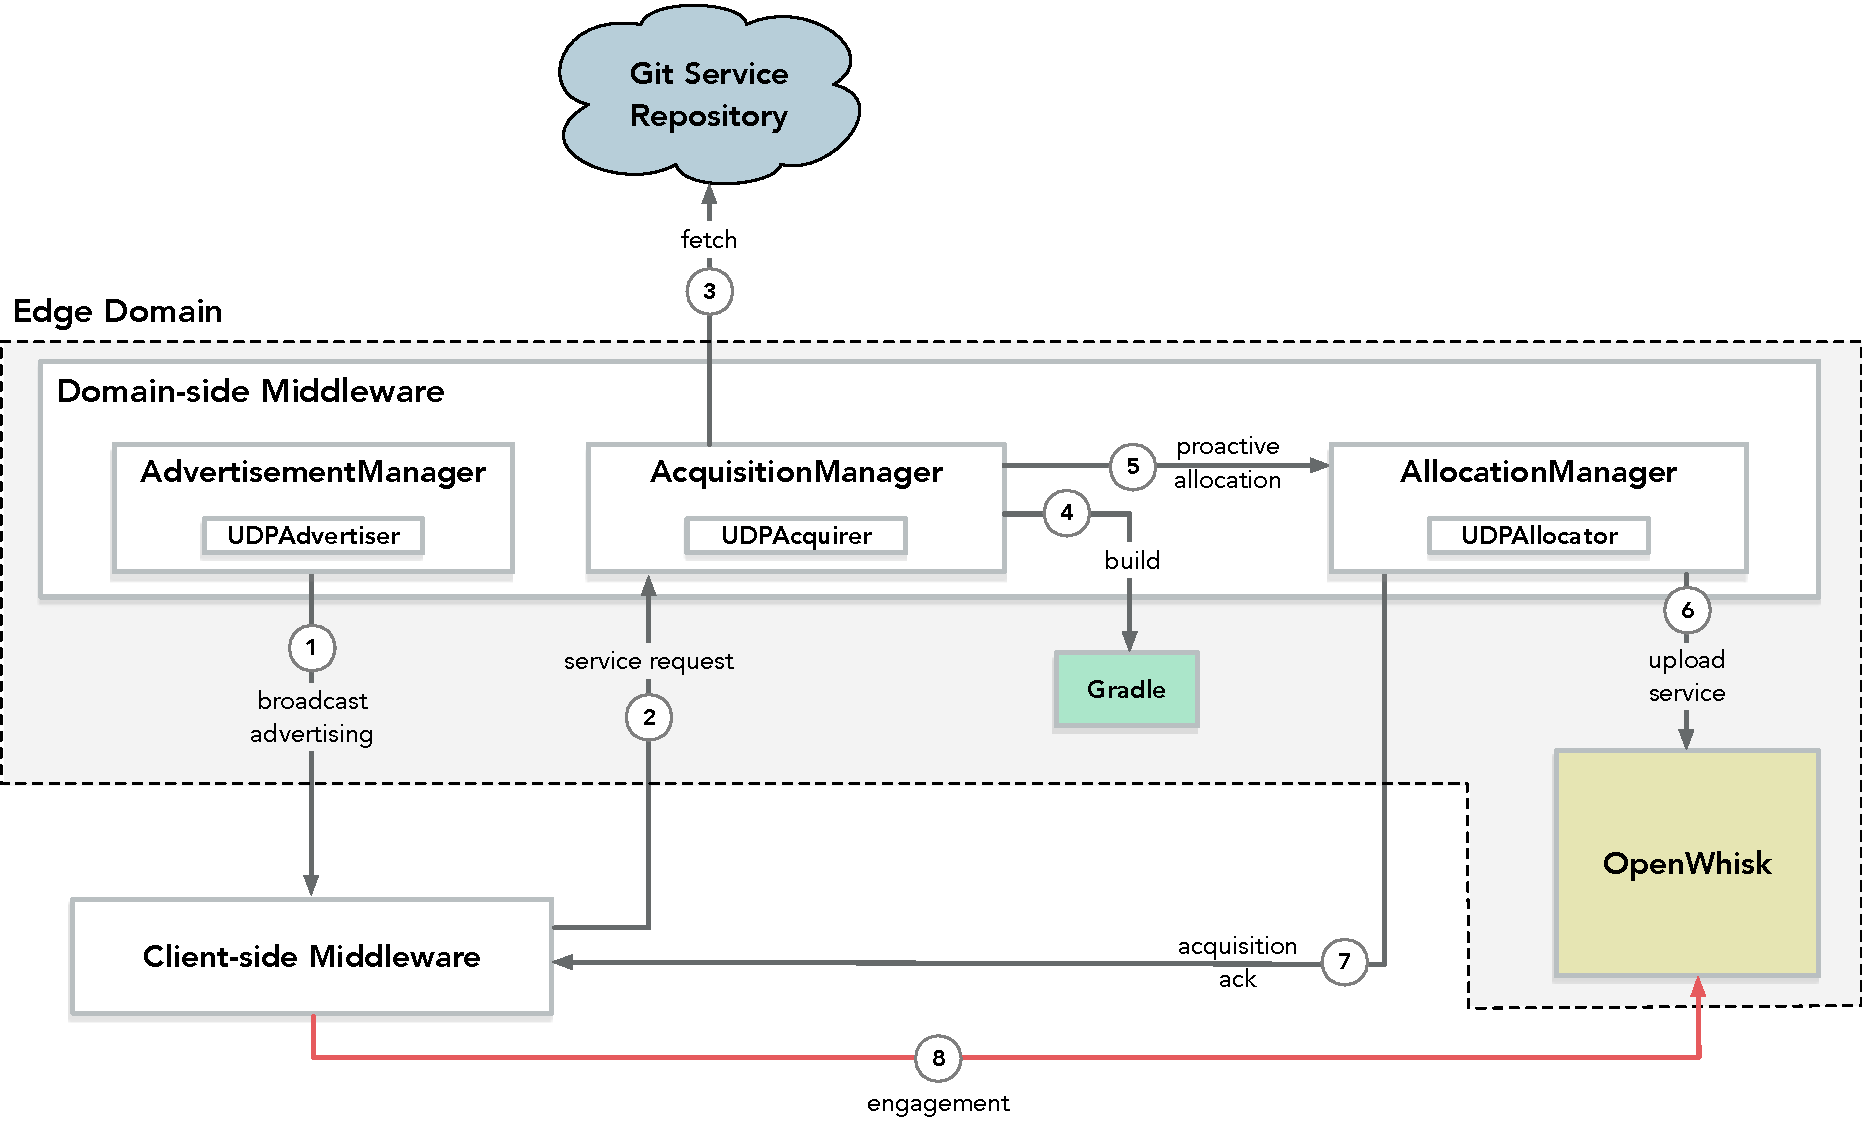
\includegraphics[width=0.9\textwidth]{figs/a3e-domain-prototype}
	\caption{Domain-side Middleware Architecture for Edge local Domain}
	\label{fig:local-edge-domain-prototype}
\end{figure}

The local-edge DSM depicted in Fig.~\ref{fig:local-edge-domain-prototype} was implemented in Python and runs within a Linux-based domain that also hosts OpenWhisk. Next, we provide a more detailed description of its implementation and behavior.

As part of the Awareness phase, an \textit{AdvertisementManager} broadcasts UDP messages (step 1) using a port that is known by the clients, with a frequency that is configurable (the default value is $5$ seconds). A unicast channel is also created through which new clients should reply (step 2) to the discovery of a domain using the address extracted from the advertisement broadcast, and a port known in advance. The CSM replies with the specification of its requested microservices (one reply per microservice) along with the public repository (e.g., Git) from which its artifacts can be downloaded.

As part of the Acquisition phase, the \textit{AcquisitionManager} downlaods (or updates existing) microservices (step 3). Among the downloaded files, a service descriptor provides information about when and how to build (step 4) source files with the microservice function(s) to be deployed to the FaaS platform. In specific, the prototype employs Gradle\footnote{\url{https://gradle.org/}} in the build process of Java functions into \textit{jar} files accepted by OpenWhisk. As an example, Listing~\ref{lst:service-descriptor} illustrates the descriptor of an image recognition service with a single Java function and two dependencies used for image classification.

Upon triggering of the Allocation phase (step 5), the \textit{AllocationManager} deploys the acquired function(s) to OpenWhisk (step 6) by means of its command-line API, and returns a message to the client-side middleware with the final endpoint of the deployed microservice along with the result of the operation (step 7). In particular, a RESTful endpoint will be created for single function in the service descriptor with the \textit{web} property assigned with value \textit{true}. From this moment on, the microservice is ready to be engaged by the client (step 8). Note that whilst the endpoint is mapped to a single function, the later may perform internal calls to other functions, effectively composing the microservice.

\definecolor{lightgrey}{gray}{0.994}
\definecolor{blue}{rgb}{0, 0, 0.25}

\lstset{
	backgroundcolor=\color{lightgrey},
	basicstyle=\footnotesize\color{black},
	string=[s]{"}{"},
	stringstyle={\footnotesize\bfseries\color{blue}},
	comment=[l]{:},
	commentstyle={\footnotesize\color{black}},
	upquote=true,
	%numbers=left,
	%numbersep=5pt,
	%numberstyle=\tiny\color{black}    
}

\begin{minipage}{.9\linewidth}
\begin{lstlisting}[caption=Image recognition service descriptor, label=lst:service-descriptor, captionpos=t]
{
 "service-name": "image-recognition",
 "functions": [{	
  "language": "Java",
   "name": "image-recognition",
   "source": "it.polimi.a3e.imagerecognition.ImageRecognition",
   "build": "true",
   "web": "true" }]
 "dependencies": ["NetSSD_deploy.prototxt", "NetSSD_deploy.caffemodel"]
}
\end{lstlisting}
\end{minipage}

\subsection{DSM Prototype: Mobile Domain}

\begin{figure}[tbp]
	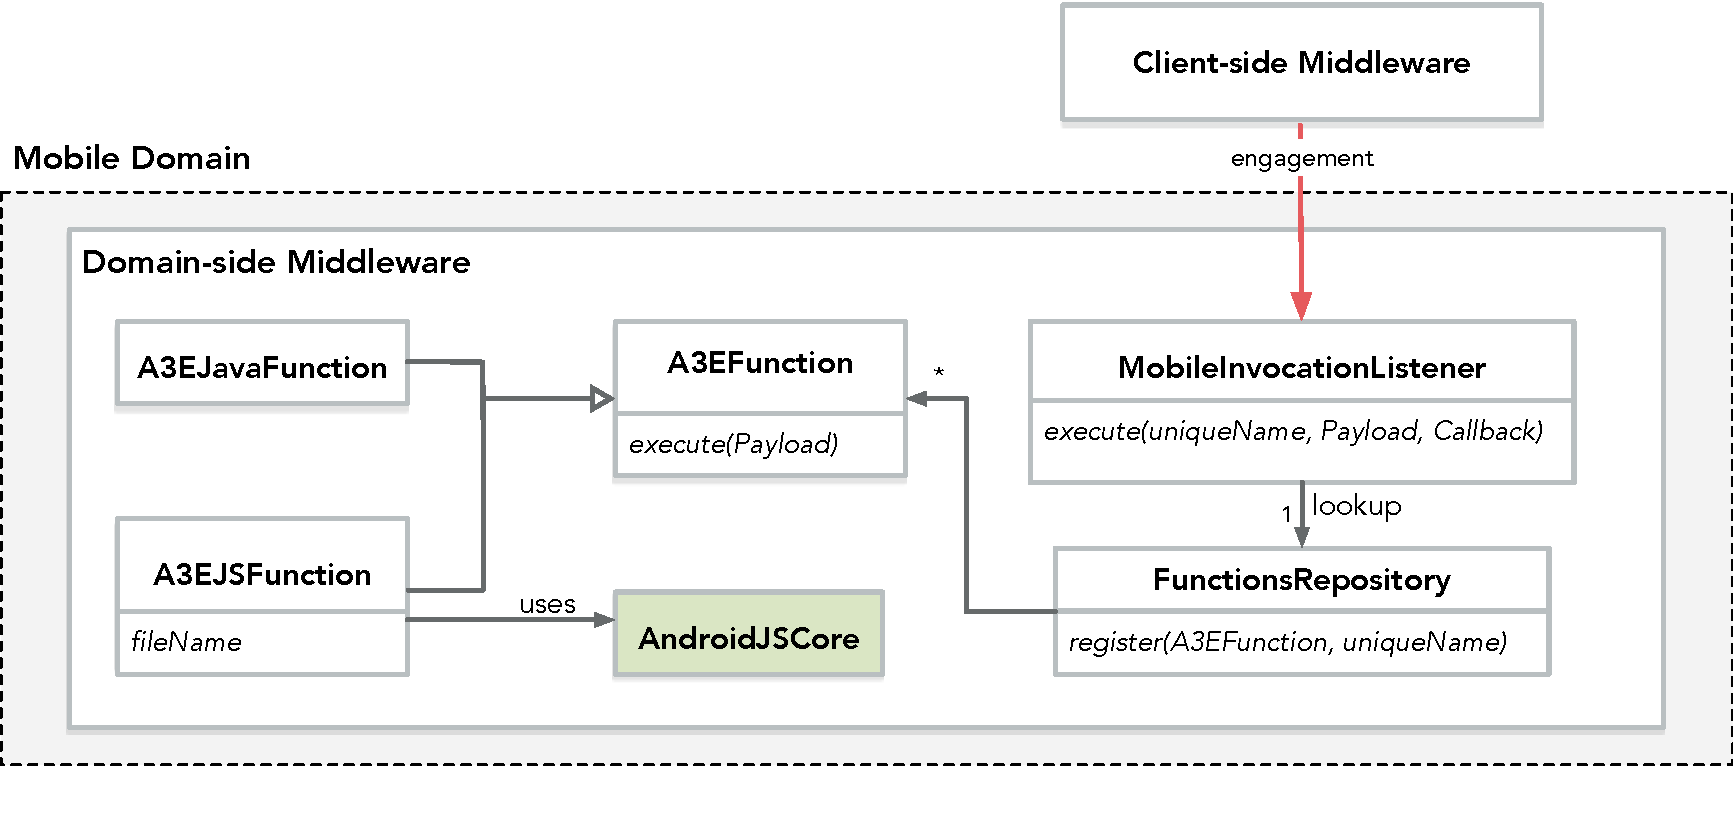
\includegraphics[width=0.9\textwidth]{figs/a3e-mobiledomain-prototype}
	\caption{Domain-side Middleware Architecture for Mobile Domain}
	\label{fig:mobile-domain-prototype}
\end{figure}

The provided mobile domain DSM prototype is depicted in Fig~\ref{fig:mobile-domain-prototype}. Next, we further detail its implementation and behavior.

%As depicted in Fig.~\ref{fig:mobile-domain-prototype}, the mobile-domain DSM implementation consists of a 
Client applications register functions to their mobile domain using component \textit{FunctionsRepository}. The prototype supports two types of functions: \textit{A3EJavaFunction} and \textit{A3EJSFunction}. In particular, \textit{A3JSFunction} represents JavaScript functions loaded from a \textit{.js} file. The latter use \textit{AndroidJSCore}~\footnote{https://github.com/ericwlange/AndroidJSCore}, an Android Java JNI wrapper required for the execution of JS code by Android applications.

The \textit{MobileInvocationListener} class handles specific Android broadcast events created by the CSM. The request is for a microservice identified by a \textit{unique name}, and is used by a \textit{FunctionsRepository} in the lookup of the corresponding \textit{A3EFunction}. For each request, the corresponding function is called with the original payload from the microservice request, which also contains a callback to be invoked as a function return.


\subsection{CSM Prototype: Android Platform}

%As described in Section~\ref{sec:proposal}, the CSM component interacts with DSM from different domains that could be either discoverable using a DNS-like mechanism or advertisement. 


\begin{figure}[tbp]
	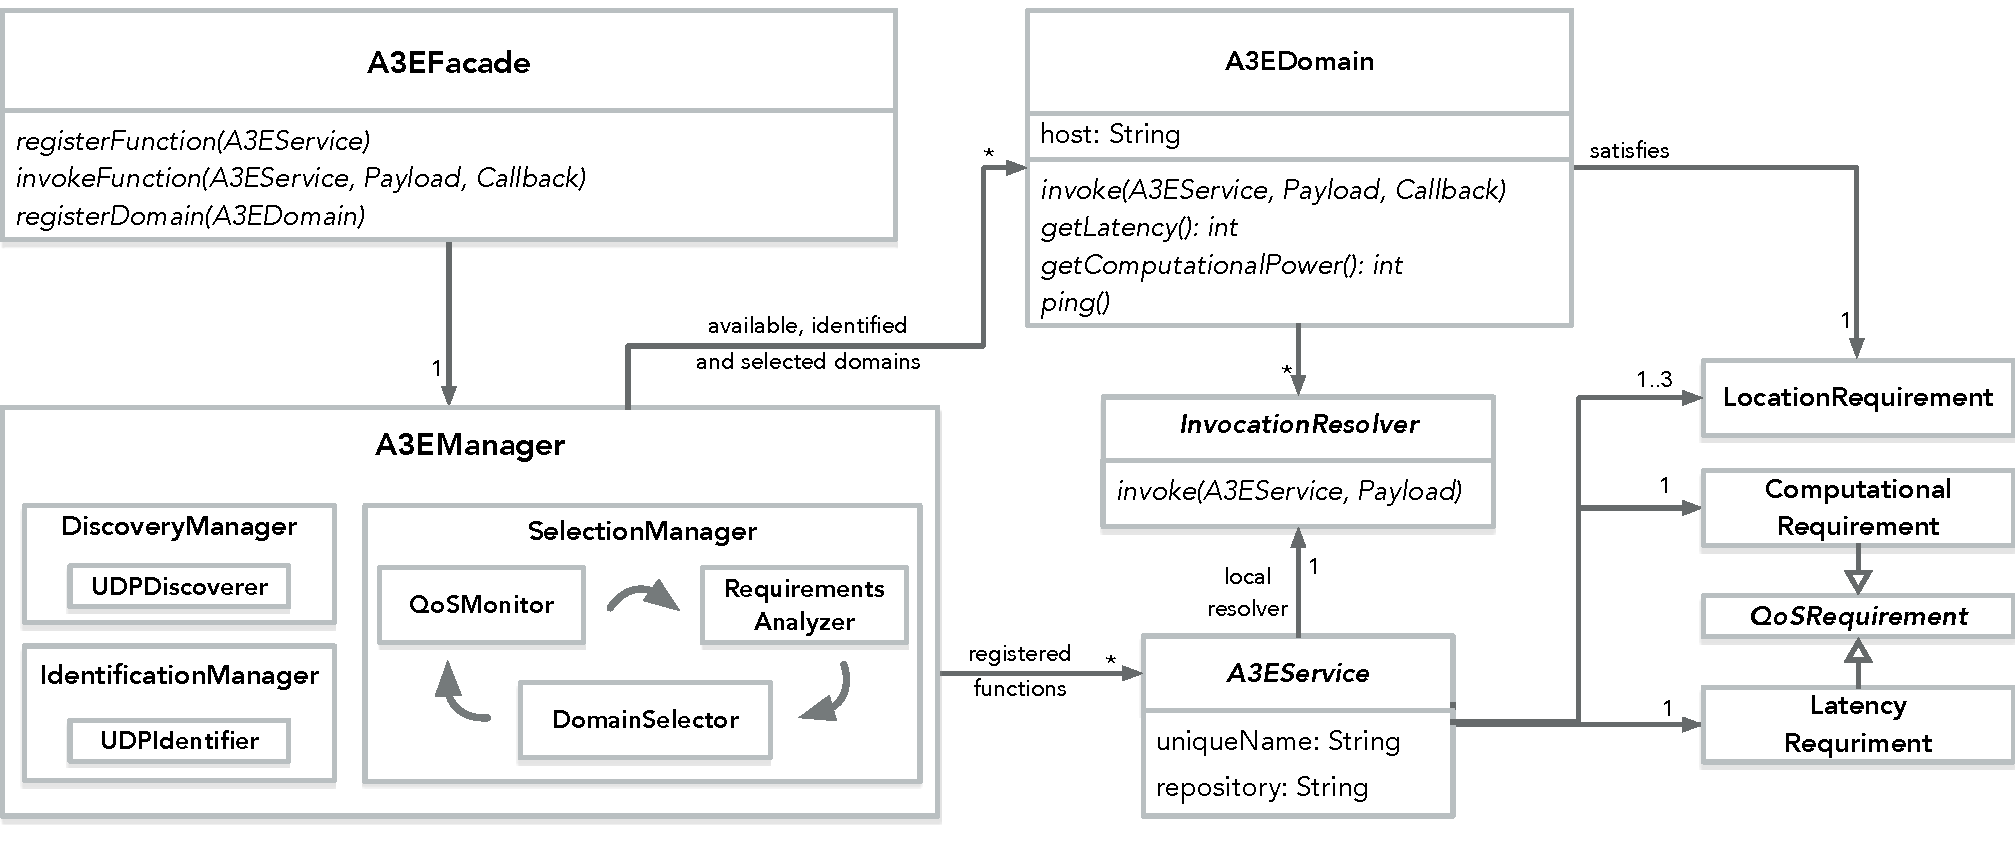
\includegraphics[width=1\textwidth]{figs/a3e-mobile-prototype}
	\caption{Client-side Middleware Architecture}
	\label{fig:mobile-prototype}
\end{figure}

Figure~\ref{fig:mobile-prototype} shows the high-level architecture of the client-side middleware. Client mobile applications interact with two components: \textit{A3EService}s and \textit{A3EFacade}. The former abstract the actual microservices to be invoked, while the latter is used to register and invoke the domain's microservices. 

An \textit{A3EService} is identified by a unique name and the url of its git code repository. It may also specify three types of requirements: 
%that corresponds to the name of the function asset that must be communicated to the continuum domains to be first acquired and then executed. Moreover each function must declare a set of non-functional QoS requirements that are organized in three types: 

\begin{enumerate}


	\item \textit{Location Requirement}s constrain where the microservice can be placed within the continuum, i.e., \textit{LOCAL}, \textit{LOCAL\_EDGE}, \textit{MOBILE\_EDGE}, or \textit{CLOUD} or a combination of the above; 


	\item a \textit{Latency Requirement} constrains network latency, i.e., \textit{ANY}, \textit{LOW} or \textit{VERY\_LOW}; and 
	

	\item a \textit{Computational Requirement} defines how relevant it is for a microservice to have fast computing, i.e., \textit{ANY}, \textit{FAST} or \textit{VERY\_ FAST}. 


\end{enumerate}

%Before becoming able for execution, the function must be registered using the \textit{A3EFacade}. 

%\begin{itemize}
	%\item \textit{Location Requirement}s are constrains over the continuum. A function can declare where it could be executed choosing a combination of three values: \textit{LOCAL}, \textit{EDGE} and \textit{CLOUD}. By default an \textit{A3EFunction} supports all three domain types but one can implement a function that, for example, cannot be executed locally thus only the \textit{EDGE} and \textit{CLOUD} requirements should be added.    
	%\item \textit{Latency Requirement} expresses how important for a function is to have a low networking latency. The default value is \textit{LOW} since the main motivation of the work is to support low-latency applications. An \textit{A3EFunction}  can  also state that this requirement should be \textit{ANY} or \textit{VERY LOW}. The lower the latency requested the more the networking latency will be considered important in the the domain selection procedure.
	%\item \textit{Computational Requirement} defines how relevant for a function is to have a fast computing processing. The predefined value is \textit{FAST}, since, again, the main targets of the approach are applications that requires fast request/response interactions. Similarly to the latency requirement two additional values are available:  \textit{ANY} or \textit{VERY FAST}. The higher  processing power is requested the more this metric will be considered important during the domain selection phase.
%\end{itemize}

%An \textit{A3EFunction} that support the \textit{LOCAL} location requirement should also define a local \textit{InvocationResolver}. As we are going to discuss later in this section, invocation resolvers deal with the invocation technology \textit{heterogenity}  of the continuum. For what regards the local domain we currently support the execution of native Java code and Javascript functions (that could be imported in the project as standard \textit{.js} files). For this purpose we created two \textit{InvocationResolver}s that can execute respectively Java or Javascript functions if the local domain is selected.

The \textit{A3EFacade} component wraps the \textit{A3EManager}, which manages all the registered \textit{A3EService}s. It consists of the discovery, identification and selection of domains, corresponding to the \textit{Awareness}, \textit{Acquisition}, and \textit{Allocation} phases of the A3-E model. 

%The loop manager consists of three main components called \textit{DiscoveryManager}, \textit{IdentificationManager} and \textit{SelectionManager}. 

Component \textit{DiscoveryManager} manages the discovery of domains. The mobile domain is registered when the CSM is instantiated, while cloud domains are registered by the client application, and their endpoints must be known a-priori. Edge domains, on the other hand, are  at run time. Every time the IP address of the client device changes, the manager starts listening for UDP broadcast messages using component \textit{UDPDiscoverer}. If a message is received within a fixed timeout of $10$ seconds, the IP address of the sender is retrieved. A new \textit{A3EDomain} is then created in the middleware and added to a list of available domains. Each \textit{A3EDomain} is identified by a \textit{host} name (URI) and satisfies a specific \textit{LocationRequirement}. 

%Everytime the connection the domain is lost, the \textit{DiscoveryManager} updates its list of available domains.

 %Component \textit{InvocationResolver} is then used to actually invoke the micro-services. 

%An  \textit{A3EDomain} could be either \textit{static} or \textit{dynamic}. Static domains are added to the discovery manager at launch time, meaning that it is known a-priori that they will be available. Example of this are cloud and local domains. On contrary dynamic domains can be found only at runtime with appropriate technological protocols (such as DNS and advertising). Edge domains are not known a-priori thus they are considered dynamic. Static domains can be added by the client application using the \textit{registerDomain} operation provided by the \textit{A3EFacade} while dynamic domains are automatically discovered by the \textit{DiscoveryManager}.
 %\textit{A3EDomain}s  are identified by a \textit{host} name, that is a unique network identifier by which it is possible to interact with the domain using a network. Moreover, as shown in the figure, a domain is considered \textit{Pingable} that means that it is possible to check for its availability and measure its networking latency (in milliseconds). Each domain satisfy a \textit{LocationRequirement}, intuitively local domains satisfies the \textit{LOCAL} requirement, while the edge and cloud ones the \textit{EDGE} and \textit{CLOUD} respectively.  A domain also provides three additional operations: one to execute a function within the domain, one to retrieve the networking latency (its value is lazily updated after a \textit{ping}) and one to obtain its computational power. Finally a domain also uses an \textit{InvocationResolver} to actually invoke the function. 


%The output of this process is the list of the available domains. 
 %This component initializes the identification phase for each new available domain (e.g., domains discovered for the first time). 

As soon as a new domain is discovered, or registered, the \textit{IdentificationManager} requests to it all the registered microservices that are executable in that domain. This is done using component \textit{UDPIndentifier}, which communicates the microservices' unique name and repository address to the domain. A microservice is not ready to be executed in the domain until a UDP confirmation message is received meaning that it is ready for the engagement phase. 

During the \textit{Engagement} phase the CSM can invoke a microservice using the \textit{invokeService} operation of the \textit{A3EFacade}. In addition to the \textit{A3EService}, the operation also expects a \textit{payload} (i.e., the function argument), and a \textit{callback} since  execution is always asynchronous. 

The \textit{A3EFacade} will retrieve the \textit{A3EDomain} that was selected for the microservice in the last control loop iteration. Since domains use heterogeneous technologies, the actual invocations are performed by the \textit{InvocationResolver} components that are bound to the different domains. 

The \textit{InvocationResolver} bound to edge and cloud domains will fire an HTTP request, while the \textit{InvocationREsolver} bound to a mobile domain will broadcast an Android event containing a request. Regardless, asynchronous \textit{callback}s are used to provide the results back to the client application. %\textit{InvocationResolver}s hide the technological details of the underlying domains. 
% bound to the domain will be used to actually \textit{execute} the function.  
%Since the control loop runs in a separated thread, the execution will not be affected if the selected domain changes during the invocation. After retrieving the best domain from the continuum, the \textit{A3EFacade} will execute the function by using the \textit{execute} operation of the \textit{A3EDomain}. Since each domains can use different technologies, the \textit{InvocationResolver} binded to the domain will be used to actually invoke the function. 
%addressing the \textit{heterogeneity} property of the continuum. 
In our current implementation of the client-side middleware we have three types of \textit{InvocationResolver}s: one for invoking microservices provided by a mobile domain, another for Rest HTTP calls (to support multiple FaaS platforms such as OpenWhisk\footnote{\url{https://github.com/apache/incubator-openwhisk/blob/master/docs/webactions.md}}), and one specifically designed for AWS Lambda\footnote{\url{https://aws.amazon.com/tools/\#sdk}}. %and finally a local invocation resolver that is binded to the local domain that simply forward the invocation to the function's local \textit{InvocationResolver} (either the \textit{JavaInvocationResolver} or \textit{JSInvocationResolver}).  


%Since each function has its own characteristics, for example different REST calls could have different \textit{content-type}s and different format for input/output, we made each function able to modify the invocation with it is own applicative details. For this reason before invoking the actual function (e.g., performing the HTTP call) the \textit{InvocationResolver} creates a technology specific \textit{InvocationMean}. These components are wrappers to technology specific objects used by the invocation resolvers to build the call (e.g., the \textit{InvokeRequest\footnote{\url{http://docs.aws.amazon.com/AWSJavaSDK/latest/javadoc/com/amazonaws/services/lambda/model/InvokeRequest.html}}} object of the AWS Lambda SDK). As shown in Figure~\ref{fig:mobile-prototype} \textit{A3EFunction}s are \textit{InvocationMeanVisitor}s. Thus, just before performing the invocation, the specific \textit{visit} method is call providing to the function a way to fill up the request for the specific type of call. 

%To summarize, supporting the continuum with A3E in a client application consists in the following four steps\footnote{A simple example of use can be found at \url{https://github.com/gioenn/a3e-android/blob/master/README.md}}:

%\begin{enumerate}
%	\item Register static \textit{A3EDomain}s such as cloud endpoints.
%	\item Create \textit{A3EFunction}s and override the specific methods to customize the requests for the technologies of interest
%	\item Register the functions
%	\item Execute the functions in the continuum as plain programmatic calls 
%\end{enumerate}